\documentclass{article}
\usepackage{graphicx} % Required for inserting images
\usepackage{float} % For [H] float placement
\usepackage{amsmath}
\usepackage{amssymb}

\usepackage{algorithmicx}
\usepackage{algorithm}
\usepackage{algpseudocode}
\title{SGP - CSP}
\author{Hamza Arharbi}
\date{January 2026}


\begin{document}

\maketitle
\tableofcontents
\newpage

\section{Introduction}



\section{Modélisation du problème Social Golfer}

Le problème du \emph{Social Golfer} consiste à répartir un ensemble de golfeurs en groupes de taille fixe sur plusieurs semaines, de sorte que chaque golfeur joue exactement une fois par semaine et que deux golfeurs ne se rencontrent jamais plus d’une fois.
Ce problème est un cas classique de problème de satisfaction de contraintes (CSP), présentant de nombreuses symétries et un espace de recherche très important.

Dans ce travail, nous proposons deux grandes familles de modélisation en MiniZinc :
\begin{itemize}
    \item une modélisation \textbf{centrée sur les groupes} ;
    \item une modélisation alternative \textbf{centrée sur les joueurs}.
\end{itemize}

Pour chacune de ces modélisations, plusieurs variantes sont étudiées : modèle de base, bris de symétries et ajout de contraintes redondantes.

\subsection{Paramètres du problème}

Les paramètres communs à tous les modèles sont :
\begin{itemize}
    \item $q$ : nombre total de golfeurs ;
    \item $g$ : nombre de groupes par semaine ;
    \item $p$ : nombre de golfeurs par groupe ;
    \item $w$ : nombre de semaines.
\end{itemize}

Une condition nécessaire à la faisabilité est imposée :
\[
q = g \times p
\]

Une borne théorique sur le nombre maximal de rencontres est également vérifiée :
\[
w \times g \times \frac{p(p-1)}{2} \leq \frac{q(q-1)}{2}
\]

Cette contrainte permet d’éliminer certaines instances irréalisables dès l’initialisation.

%--------------------------------------------------
\subsection{Modélisation 1 : Vue par groupes}

\subsubsection{Variables de décision}

Dans cette première approche, les variables représentent directement les groupes formés chaque semaine.

\[
\texttt{Groupes}[s,g] \subseteq \texttt{GOLFEURS}
\]

où \texttt{Groupes[$s,g$]} est l’ensemble des golfeurs affectés au groupe $g$ de la semaine $s$.
Les variables sont donc des variables ensemblistes.

\subsubsection{Contraintes communes}

Les contraintes suivantes sont présentes dans toutes les variantes de cette modélisation.

\paragraph{Taille des groupes}
Chaque groupe contient exactement $p$ golfeurs :
\[
\forall s,g,\quad |\texttt{Groupes}[s,g]| = p
\]

\paragraph{Unicité par semaine}
Un golfeur ne peut appartenir qu’à un seul groupe par semaine :
\[
\forall s,\quad \texttt{all\_disjoint}(\{\texttt{Groupes}[s,g]\}_{g})
\]

\paragraph{Contrainte sociale}
Deux golfeurs ne peuvent jouer ensemble qu’une seule fois :
\[
\forall s_1 < s_2,\forall g_1,g_2,\quad
|\texttt{Groupes}[s_1,g_1] \cap \texttt{Groupes}[s_2,g_2]| \leq 1
\]

\subsubsection{Modèle de base}

Le modèle \texttt{base.mzn} implémente uniquement les contraintes fondamentales.
Bien que correct, ce modèle souffre d’un grand nombre de symétries :
\begin{itemize}
    \item permutation des golfeurs ;
    \item permutation des groupes ;
    \item permutation des semaines.
\end{itemize}

Ces symétries entraînent une exploration redondante de l’espace de recherche.

\subsubsection{Bris de symétrie simple}

Le modèle \texttt{base\_symetri\_simple.mzn} introduit un premier bris de symétrie en fixant complètement la première semaine.  
L’idée est que, sans cette contrainte, la permutation des golfeurs et des groupes dans la première semaine générerait de multiples solutions équivalentes.

La contrainte introduite peut s’écrire mathématiquement comme suit :

\[
\forall j \in \{1, \dots, g\}, \quad
\texttt{Groupes}[1,j] = \{ (j-1)p + 1, \dots, j \cdot p \}
\]

Autrement dit, le premier groupe contient les joueurs $1$ à $p$, le deuxième groupe $p+1$ à $2p$, et ainsi de suite.  

\noindent
\textbf{Effet :} Cette contrainte :
\begin{itemize}
    \item élimine toutes les solutions obtenues par permutation des golfeurs dans la première semaine ;
    \item élimine toutes les solutions obtenues par permutation des groupes dans la première semaine ;
    \item réduit considérablement l’espace de recherche du solveur sans enlever de solutions réalisables.
\end{itemize}



\subsubsection{Bris de symétries complet}

Le modèle \texttt{base\_symetri.mzn} va plus loin en introduisant des contraintes de bris de symétries supplémentaires sur les semaines suivantes :

\paragraph{1. Ordre lexicographique des groupes dans chaque semaine}
Pour toute semaine $i \ge 2$, on impose un ordre lexicographique entre les groupes afin d’éviter les permutations équivalentes :

\[
\forall i \in \{2, \dots, w\}, \quad \forall j \in \{1, \dots, g-1\}, \quad
\texttt{Groupes}[i,j] \prec \texttt{Groupes}[i,j+1]
\]

où $\prec$ représente l’ordre lexicographique des ensembles de golfeurs.

\paragraph{2. Ordre des semaines}
On impose également un ordre entre les semaines basé sur le premier groupe :

\[
\forall i \in \{2, \dots, w-1\}, \quad
\texttt{Groupes}[i,1] \prec \texttt{Groupes}[i+1,1]
\]

\noindent
\textbf{Effet :} Ces contraintes éliminent toutes les solutions obtenues par permutation :
\begin{itemize}
    \item des groupes au sein d’une même semaine ;
    \item des semaines elles-mêmes.
\end{itemize}


\subsubsection{Contraintes redondantes}

Le modèle \texttt{base\_redondant.mzn} introduit des contraintes supplémentaires pour améliorer la propagation, sans changer l’ensemble des solutions valides.

\paragraph{1. Matrice des rencontres}
On définit une matrice auxiliaire $Rencontres[i,j] \in \{0,1\}$ qui indique si le joueur $i$ a rencontré le joueur $j$ au moins une fois.  

\[
Rencontres[i,j] = 
\begin{cases}
1 & \text{si } \exists s,g \text{ tel que } \{i,j\} \subseteq \texttt{Groupes}[s,g] \\
0 & \text{sinon}
\end{cases}
\]

Cette contrainte est liée aux variables \texttt{Groupes} par un \emph{channeling} :

\[
\forall i < j,\quad Rencontres[i,j] = \text{bool2int} \Big( \bigvee_{s,g} ( \{i,j\} \subseteq \texttt{Groupes}[s,g] ) \Big)
\]

\paragraph{2. Symétrie de la matrice et diagonale}
\[
Rencontres[i,j] = Rencontres[j,i], \quad \forall i,j
\]
\[
Rencontres[i,i] = 0, \quad \forall i
\]

\paragraph{3. Contrainte sur le nombre exact de rencontres}
Chaque joueur doit rencontrer exactement $w(p-1)$ adversaires distincts :

\[
\forall i,\quad \sum_{j \in GOLFEURS} Rencontres[i,j] = w \cdot (p-1)
\]

\noindent
\textbf{Effet :} Cette contrainte redondante permet :
\begin{itemize}
    \item de détecter plus rapidement les conflits dans l’assignation des groupes ;
    \item d’améliorer la propagation des contraintes et de réduire l’espace de recherche ;
    \item de garantir que chaque joueur a rencontré exactement le nombre requis d’adversaires.
\end{itemize}



%--------------------------------------------------
\subsection{Modélisation 2 : Vue par joueurs}

\subsubsection{Principe}

La seconde modélisation adopte un point de vue inversé.
Chaque golfeur est associé aux groupes (appelés \emph{slots}) auxquels il participe.

Un slot correspond à un couple (semaine, groupe) et est représenté par un entier.

\subsubsection{Variables de décision}

\[
\texttt{Planning\_Joueur}[j] \subseteq \texttt{SLOTS}
\]

où \texttt{Planning\_Joueur[$j$]} représente l’ensemble des groupes auxquels participe le joueur $j$.

\subsubsection{Contraintes}

\paragraph{Participation hebdomadaire}
Chaque joueur joue exactement une fois par semaine :
\[
|\texttt{Planning\_Joueur}[j]| = w
\]

\paragraph{Taille des groupes}
Chaque slot doit contenir exactement $p$ joueurs :
\[
\sum_j [k \in \texttt{Planning\_Joueur}[j]] = p
\]

\paragraph{Contrainte sociale}
Deux joueurs ne partagent au plus qu’un seul slot :
\[
|\texttt{Planning\_Joueur}[j_1] \cap \texttt{Planning\_Joueur}[j_2]| \leq 1
\]

\subsubsection{Bris de symétries}

Dans la modélisation par joueurs (\texttt{base2\_redondant.mzn}), le bris de symétries est appliqué aux \emph{slots} de chaque joueur pour réduire l’espace de recherche :

\paragraph{1. Fixation de la semaine 1}
Chaque joueur $j$ est assigné à un slot spécifique dans la première semaine, ce qui fixe complètement la configuration initiale :

\[
\forall j \in \{1, \dots, q\}, \quad \left\lfloor \frac{j-1}{p} \right\rfloor + 1 \in Planning\_Joueur[j]
\]

\paragraph{2. Fixation du joueur 1}
Le joueur 1 est utilisé comme étalon pour toutes les semaines afin de casser les symétries liées aux permutations de joueurs et de groupes dans les semaines suivantes :

\[
Planning\_Joueur[1] = \{ k \cdot g + 1 \mid k = 0, \dots, w-1 \}
\]

\noindent
\textbf{Effet :} Ces contraintes empêchent les solutions équivalentes obtenues par permutation des joueurs ou des slots, réduisant ainsi l’espace de recherche pour le solveur.

\subsubsection{Contraintes redondantes}

En complément du bris de symétries, des contraintes redondantes sont introduites pour améliorer la propagation et la faisabilité sociale.

\paragraph{Contrainte de rencontre globale}
On vérifie que chaque joueur rencontre exactement $w(p-1)$ adversaires distincts via les slots :

\[
\forall j_1 \in GOLFEURS, \quad
\sum_{j_2 \in GOLFEURS, j_2 \neq j_1} |Planning\_Joueur[j_1] \cap Planning\_Joueur[j_2]| = w \cdot (p-1)
\]

\noindent
\textbf{Effet :} Cette contrainte :
\begin{itemize}
    \item accélère la propagation des contraintes dans le solveur ;
    \item réduit l’espace de recherche en détectant plus rapidement les conflits ;
    \item garantit que chaque joueur rencontre exactement le nombre requis d’adversaires distincts.
\end{itemize}


\section{Solveur ensembliste}

\subsection{Fonctionnement du solveur ensembliste}

Le solveur repose sur un mécanisme de \emph{backtracking} combiné à la propagation des contraintes et à l'apprentissage de \emph{nogoods}. 
Le processus global peut se décrire comme suit :

\begin{enumerate}
    \item \textbf{Vérification des nogoods :} 
    Avant d'explorer un chemin, le solveur vérifie si celui-ci correspond à un chemin déjà identifié comme impossible (nogood). 
    Si c'est le cas, il effectue un backtrack immédiat.

    \item \textbf{Restart :} 
    Si la profondeur maximale est atteinte, le solveur peut réinitialiser l'état des variables et relancer la recherche.

    \item \textbf{Propagation des contraintes :} 
    À chaque étape, les opérations appliquées sur les variables sont utilisées pour reconstruire l'état courant et propager toutes les contraintes jusqu'à stabilisation.

    \item \textbf{Vérification de solution :} 
    Si toutes les contraintes sont satisfaites par l'état courant, la solution est retournée.

    \item \textbf{Choix de la variable et de la valeur :} 
    Le solveur sélectionne une variable non déterminée selon une heuristique (par exemple MRV, nombre de contraintes, ou aléatoire), 
    puis choisit une valeur à essayer pour cette variable.

    \item \textbf{Backtracking :} 
    Pour chaque valeur sélectionnée, le solveur tente d'ajouter cette valeur au lower bound de la variable. 
    Si aucun chemin ne conduit à une solution, il retire cette valeur (upper bound) et explore d'autres options. 
    Si toutes les possibilités sont épuisées, un \emph{nogood} est appris et le solveur revient en arrière.

\end{enumerate}
\begin{figure}[H]
    \centering
    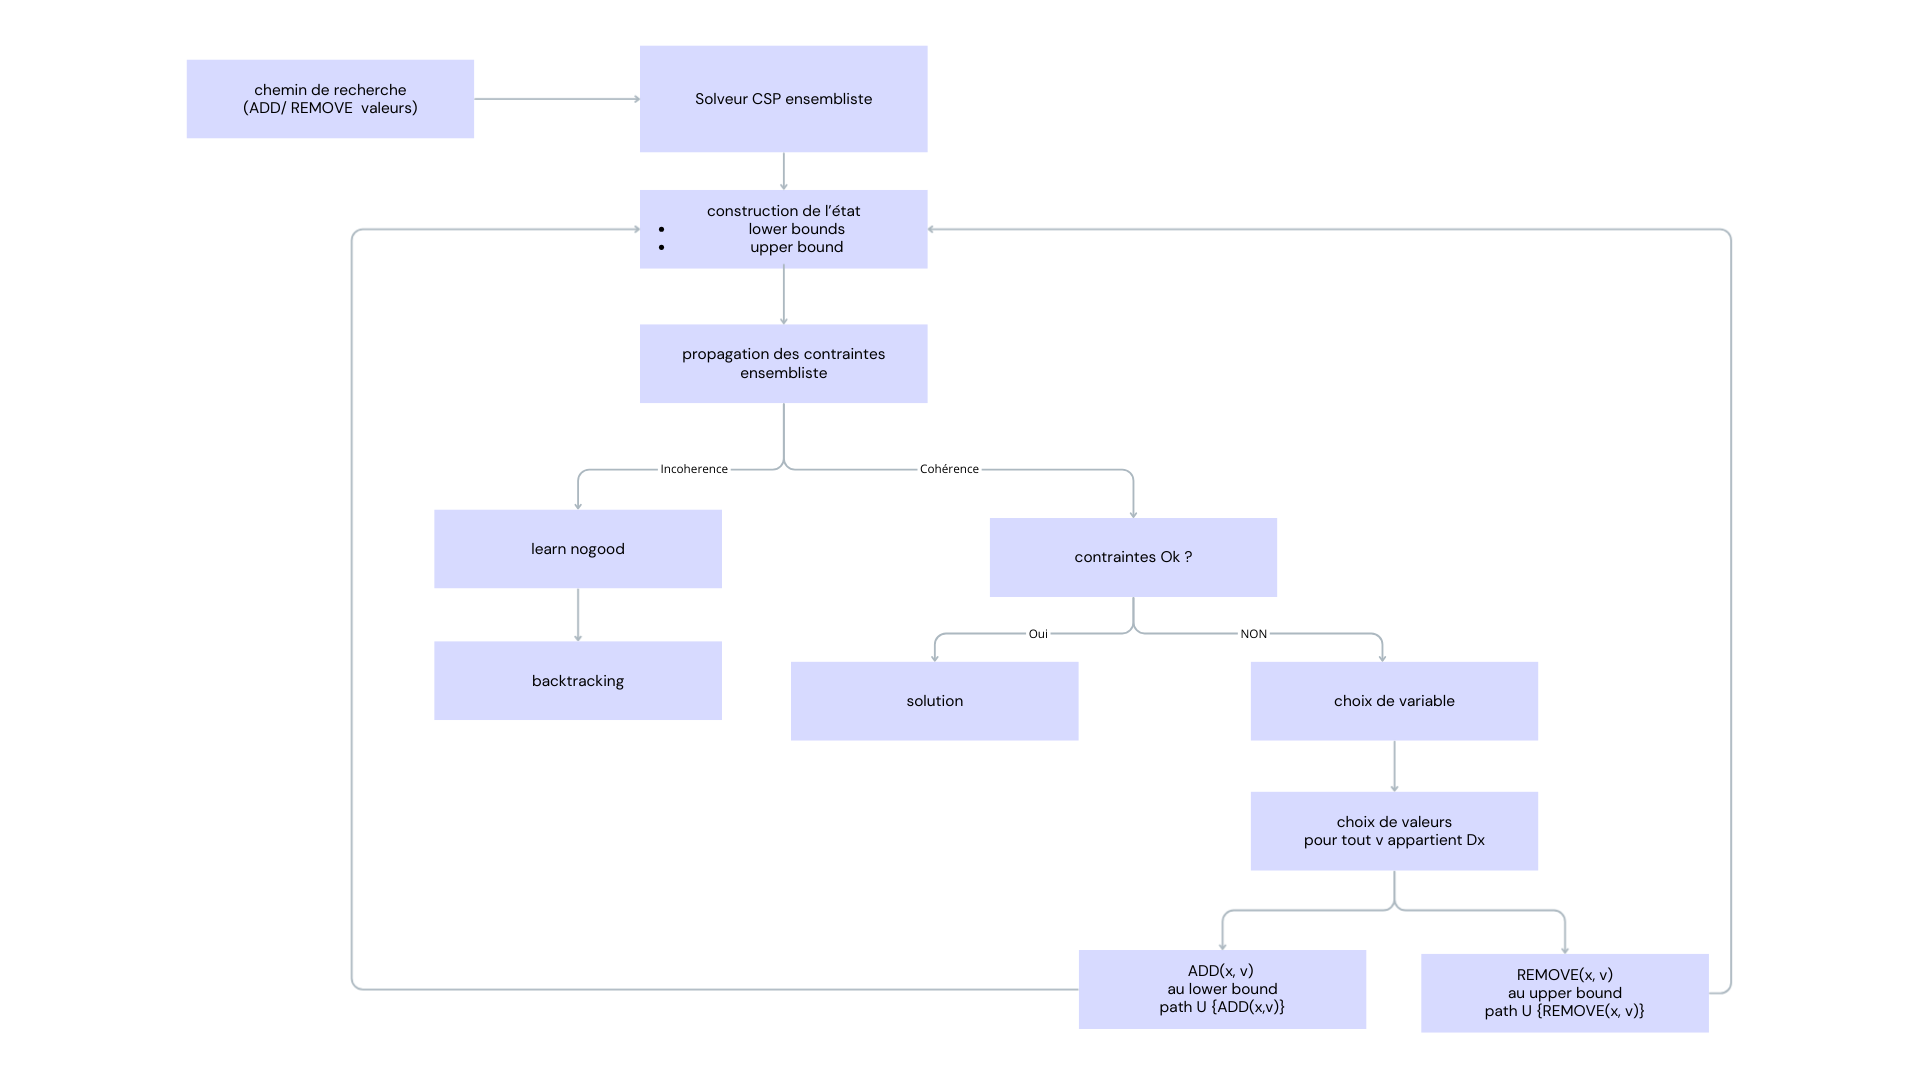
\includegraphics[width=0.8\textwidth]{2.png}
    \caption{Architecture du solveur ensembliste}
    \label{fig:monimage}
\end{figure}
Ce mécanisme permet au solveur d'explorer efficacement l'espace combinatoire tout en évitant de répéter des chemins déjà identifiés comme impossibles, et en profitant de la propagation des contraintes pour réduire l'espace de recherche.

\subsection{Algorithme du solveur}

\begin{algorithm}[H]
\caption{Solveur CSP ensembliste}
\label{alg:set_solver}
\begin{algorithmic}[1]

\Function{Solve}{}
    \While{true}
       \If{Search renvoie RestartException}
            \State \textbf{continue}
        \Else
            \State \Return \Call{Search}{$\emptyset$}
        \EndIf
    \EndWhile
\EndFunction
\newline
\newline
\Function{Search}{$path$}
    \If{\Call{IsNogood}{$path$} \textbf{or} \Call{RestartCriterion}{}}
        \State \Return \textbf{None}
    \EndIf

    \State $state \gets$ \Call{BuildState}{$path$}
    \If{$state$ incohérent}
        \State \Call{LearnNogood}{$path$}
        \State \Return \textbf{None}
    \EndIf

    \If{\Call{AllConstraintsSatisfied}{$state$}}
        \State \Return \Call{ExtractSolution}{$state$}
    \EndIf

    \State $(x, D_x) \gets$ \Call{ChooseVariable}{$state$}
    \ForAll{$v \in$ \Call{ChooseValues}{$D_x$}}
        \State $sol \gets$ \Call{Search}{$path \cup \{\textsc{Add}(x,v)\}$}
        \If{$sol \neq$ \textbf{None}} \State \Return $sol$ \EndIf
        \State $sol \gets$ \Call{Search}{$path \cup \{\textsc{Remove}(x,v)\}$}
        \If{$sol \neq$ \textbf{None}} \State \Return $sol$ \EndIf
    \EndFor

    \State \Call{LearnNogood}{$path$}
    \State \Return \textbf{None}

\EndFunction

\end{algorithmic}
\end{algorithm}




\subsection{Variables ensemblistes}
Dans ce solveur, chaque variable est modélisée comme un \textbf{ensemble de valeurs possibles}, plutôt que comme une valeur unique. 
L'idée centrale est de maintenir \textbf{deux bornes} pour chaque variable :

\begin{itemize}
    \item \textbf{Lower bound (borne inférieure)} : ensemble des valeurs qui sont \emph{déjà certaines} pour cette variable. 
    Toute valeur présente dans le lower bound fait partie de la solution finale. 
    Le lower bound ne peut jamais contenir de valeur absente du upper bound.

    \item \textbf{Upper bound (borne supérieure)} : ensemble des valeurs \emph{encore possibles} pour cette variable. 
    Toute valeur présente dans l'upper bound peut potentiellement faire partie de la solution. 
    L'upper bound évolue au fur et à mesure de la propagation des contraintes et des choix effectués pendant la recherche.
\end{itemize}

Une variable est dite \textbf{déterminée} lorsque son lower bound et son upper bound \emph{coïncident exactement}. 
À ce stade, la valeur de la variable est entièrement fixée et ne peut plus évoluer.

Le solveur fonctionne en \textbf{réduisant progressivement les domaines des variables} :
\begin{itemize}
    \item lorsqu'une valeur est confirmée pour une variable, elle est ajoutée au lower bound ;
    \item lorsqu'une valeur est impossible, elle est retirée de l'upper bound.
\end{itemize}

Cette approche permet de \textbf{séparer les décisions certaines et possibles}, ce qui facilite la propagation des contraintes, le backtracking et l'apprentissage de nogoods.

Enfin, chaque variable conserve une \textbf{copie de ses bornes initiales}, ce qui permet de la \emph{réinitialiser facilement} lors d'un restart, garantissant que l'état initial est toujours récupérable.



\subsection{Contraintes ensemblistes}

Le solveur utilise différents types de contraintes pour propager les informations et réduire les domaines des variables. Chaque contrainte agit sur un ou plusieurs ensembles de valeurs et permet de vérifier la cohérence des assignations.

\begin{itemize}
    \item \textbf{Union} : cette contrainte assure que l'ensemble résultat est la \emph{réunion} des ensembles des variables concernées. 
    
    \textbf{Règle de filtrage} : 
    \begin{itemize}
        \item la borne supérieure du résultat est réduite pour contenir uniquement les valeurs possibles dans au moins une variable,
        \item la borne inférieure du résultat est augmentée pour inclure toutes les valeurs déjà certaines dans les variables.
    \end{itemize}


    \item \textbf{Intersection} : cette contrainte garantit que l'ensemble résultat est l'\emph{intersection} des ensembles des variables concernées. 
    
    \textbf{Règle de filtrage} : 
    \begin{itemize}
        \item la borne inférieure du résultat est augmentée pour inclure uniquement les valeurs certaines dans toutes les variables,
        \item la borne supérieure du résultat est réduite pour contenir uniquement les valeurs possibles dans toutes les variables.
    \end{itemize}

    \item \textbf{Subset} : cette contrainte impose qu'un ensemble soit un \emph{sous-ensemble} d'un autre ($\text{var1} \subseteq \text{var2}$). Tous les éléments de var1 doivent obligatoirement être dans var2.

    \textbf{Règle de filtrage} : 
    \begin{itemize}
        \item la borne supérieure de var1 est réduite à l'intersection avec la borne supérieure de var2 (var1 ne peut contenir que ce qui est possible dans var2),
        \item la borne inférieure de var2 est augmentée pour inclure la borne inférieure de var1 (si un élément est certain dans var1, il doit être certain dans var2).
    \end{itemize}

    \item \textbf{Different} : cette contrainte impose que deux ensembles soient \emph{distincts} ($\text{var1} \neq \text{var2}$). Les deux variables ne peuvent pas être égales.
    \textbf{Règle de filtrage} : 
    \begin{itemize}
        \item une incohérence est détectée immédiatement si les deux variables sont complètement déterminées et possèdent exactement les mêmes éléments,
        \item tant que les variables ne sont pas entièrement déterminées, la contrainte peut potentiellement être satisfaite par des choix divergents.
    \end{itemize}


    \item \textbf{CardinalityConstraint} : cette contrainte impose qu'une variable contienne exactement un nombre donné d'éléments. 

    \textbf{Règle de filtrage} : 
    \begin{itemize}
        \item si le nombre de valeurs certaines atteint la cardinalité, toutes les autres valeurs possibles sont retirées de la borne supérieure,
        \item si le nombre de valeurs restantes possibles est exactement ce qui manque pour atteindre la cardinalité, elles sont ajoutées à la borne inférieure.
    \end{itemize}


    \item \textbf{IntersectionCardinalityConstraint} : cette contrainte limite le nombre d'éléments communs entre les ensembles de deux variables. 
    
    \textbf{Règle de filtrage} : 
    \begin{itemize}
        \item toute valeur qui, si ajoutée à la borne inférieure d'une variable, ferait dépasser le maximum d'intersection autorisé est retirée de la borne supérieure,
        \item une incohérence est détectée immédiatement si l'intersection des bornes inférieures dépasse la limite.
    \end{itemize}
\end{itemize}

Ces contraintes permettent au solveur de propager efficacement les informations, de réduire l'espace de recherche et de détecter rapidement les chemins impossibles, facilitant ainsi le backtracking et l'apprentissage de nogoods.


\subsection{Heuristiques}
\subsubsection{Heuristique de choix de variable}

Le solveur utilise différentes stratégies pour sélectionner la prochaine variable non déterminée sur laquelle effectuer une assignation. 
Le but de cette heuristique est de guider la recherche vers les variables les plus prometteuses, afin de réduire l'espace de recherche et d'augmenter l'efficacité du backtracking.

\begin{itemize}
    \item \textbf{Variables non déterminées} : seules les variables dont le lower bound est différent de l'upper bound sont candidates au choix.

    \item \textbf{Stratégies de sélection} :
    \begin{itemize}
        \item \textbf{Random} : une variable est choisie aléatoirement parmi les non-déterminées.
        \item \textbf{Minimum Remaining Values (MRV)} : la variable avec le plus petit nombre de valeurs encore possibles (upper bound moins lower bound) est sélectionnée, afin de traiter d'abord les variables les plus contraignantes.
        \item \textbf{Least Constraints} : la variable impliquée dans le moins de contraintes est sélectionnée, pour réduire le risque de propagation immédiate d'incohérences.
        \item \textbf{Most Constraints} : la variable impliquée dans le plus de contraintes est sélectionnée, pour maximiser l'effet de propagation et détecter tôt les conflits.
    \end{itemize}

    \item \textbf{Randomisation et prévention des minima locaux} :
    Pour éviter de rester bloqué dans des minima locaux, le solveur peut sélectionner aléatoirement une variable parmi les $K$ premières du classement selon la stratégie choisie après un certain nombre de choix consécutifs.

    \item \textbf{Restart automatique} :
    Si la profondeur de recherche maximale est atteinte, un \emph{restart} est déclenché, réinitialisant les variables et l'état de recherche.
\end{itemize}

Cette heuristique permet de combiner exploitation (traiter les variables les plus critiques) et exploration (randomisation), améliorant l'efficacité du solveur ensembliste.




\subsubsection{Heuristique de choix de valeur}

Une fois la variable sélectionnée, le solveur choisit l'ordre dans lequel tester ses valeurs possibles. 
Les valeurs considérées sont celles présentes dans l'upper bound mais pas encore dans le lower bound.

\begin{itemize}
    \item \textbf{Random} : les valeurs sont mélangées aléatoirement afin d'explorer l'espace de recherche sans biais.
    
    \item \textbf{Least Used / Minimum Occurrences} : les valeurs sont triées selon le nombre de fois où elles ont déjà été assignées précédemment à la variable. 
    Les valeurs les moins utilisées sont essayées en premier, ce qui favorise la diversification de la recherche et réduit le risque de cycles.
\end{itemize}

Cette stratégie permet de combiner exploitation et exploration :  
- l'exploration par la randomisation aide à sortir des minima locaux,  
- l'exploitation via le comptage d'occurrences favorise l'utilisation des valeurs moins testées, équilibrant ainsi la recherche.


\subsubsection{Nogoods}

Les \emph{nogoods} sont des chemins ou des assignations partiels connus comme étant impossibles. 
Ils permettent au solveur de \textbf{détecter rapidement les échecs récurrents} et d'éviter de réexplorer des sous-arbres inutiles.

\begin{itemize}
    \item \textbf{Apprentissage des nogoods} : lorsqu'un chemin de recherche mène à un échec (aucune assignation ne peut satisfaire toutes les contraintes), ce chemin est transformé en nogood.

    \item \textbf{Vérification} : avant de continuer l'exploration d'un chemin, le solveur vérifie si le chemin courant correspond à un nogood existant. 
    Si c'est le cas, la recherche est interrompue immédiatement, permettant un \textbf{backtracking anticipé}.

    \item \textbf{Objectif} : cette approche réduit significativement l'espace de recherche, car elle empêche la répétition des mêmes erreurs, et améliore l'efficacité du solveur ensembliste.
\end{itemize}

\subsubsection{Construction de l'état à partir du chemin de recherche}

Le solveur représente l'état courant des variables ensemblistes en appliquant successivement les \emph{opérations} effectuées le long du chemin de recherche. 
Chaque opération correspond soit à l'ajout d'une valeur au \emph{lower bound} d'une variable, soit à la suppression d'une valeur de son \emph{upper bound}.

\begin{itemize}
    \item \textbf{Application des opérations} : pour chaque opération du chemin, le solveur met à jour les bornes inférieures et supérieures des variables concernées. 
    Cette mise à jour reflète toutes les décisions prises jusqu'à ce point dans l'exploration.

    \item \textbf{Propagation des contraintes} : après chaque mise à jour, toutes les contraintes sont appliquées de manière itérative jusqu'à ce qu'aucune nouvelle réduction ne soit possible. 
    Cela permet de propager les implications des décisions prises et de détecter rapidement les incohérences.

    \item \textbf{Caching} : chaque état calculé est mis en cache. 
    Si un même chemin est rencontré ultérieurement, le solveur peut réutiliser l'état déjà calculé, évitant ainsi des recalculs coûteux et accélérant la recherche.
\end{itemize}

Cette construction systématique de l'état à partir des opérations garantit que le solveur maintient toujours une représentation cohérente des variables et de leurs domaines, facilitant la propagation, le backtracking et l'apprentissage de nogoods.

\subsubsection{Caching}

Pour améliorer l'efficacité de la recherche, le solveur utilise un mécanisme de \emph{caching} des états intermédiaires. 
Chaque chemin de recherche est représenté par la séquence d'opérations appliquées aux variables. 

\begin{itemize}
    \item Lorsqu'un chemin est exploré pour la première fois, l'état correspondant (i.e. les bornes inférieure et supérieure de toutes les variables) est calculé en appliquant toutes les opérations du chemin et en effectuant la propagation des contraintes jusqu'à stabilisation.
    
    \item L'état résultant est stocké dans un cache associant la représentation du chemin à l'état complet. 

    \item Si le même chemin est rencontré à nouveau, le solveur peut récupérer directement l'état depuis le cache, évitant ainsi de recalculer les mises à jour des variables et la propagation des contraintes. 

    \item Ce mécanisme réduit le temps de calcul, en particulier lorsque certains sous-arbres de l'espace de recherche sont visités plusieurs fois.
\end{itemize}

Ainsi, le caching permet d'optimiser le backtracking en minimisant les recalculs et en accélérant la détection des inconsistances.


\subsection{Résultats expérimentaux}

Les performances du solveur ensembliste ont été évaluées sur plusieurs instances du problème Social Golfer. 
Le tableau ci-dessous présente le temps de résolution pour chaque instance.

\begin{table}[H]
\centering
\begin{tabular}{|c|c|c|c|c|c}
\hline
\textbf{Semaines (W)} & \textbf{Groupes (G)} & \textbf{Joueurs par groupe (P)} & \textbf{Instance} & \textbf{Temps de résolution (s)} \\
\hline
2 & 2 & 2 & W2G2P2 & 0,053 \\
\hline
3 & 3 & 2 & W3G3P2 & 0,072 \\
\hline
4 & 3 & 2 & W4G3P2 & 0,085 \\
\hline
4 & 3 & 3 & W4G3P3 & 0,089 \\
\hline
4 & 2 & 3 & W4G2P3 & ----- \\
\hline
\end{tabular}
\caption{Temps de résolution des différentes instances du solveur ensembliste.}
\label{tab:resultats}
\end{table}



\end{document}
